%# -*- coding:utf-8 -*-
\begin{ack}
% 2021年的某一天,我偶然地翻到了一篇文章\ucite{zhang2021dynamic},文章大致内容是通过张量建模推荐系统的时间动力学云云,其中涉及了很多统计学和数值分析的知识。由于我甚至没有接受过系统的基础数学教育\footnote{我是电子系出身,念研究生之前学校只教过两学期的所谓高等数学,一学期的线性代数和一学期的概率论与数理统计,而且我当时又喜欢逃课。},所以以我的水平并不是很懂,并且那时我更倾向于把时间花在优化上,因此也就是随便翻翻罢了。一句话吸引了我的注意:
% \begin{quote}
% 	To solve the objective function (3), we incorporate the maximum block improvement (MBI) strategy (Chen \textit{et al.}, 2012) into the BCD algorithm cyclically as in Bi \textit{et al.} (2018).
% \end{quote}
% 我觉得很震撼,这种震撼难以言表。我转念想到,做出这样优秀工作\ucite{chen2012maximum}的人,竟恰好是我的指导老师。我多么够运。

首先,我想感谢我的指导老师陈碧连副教授。感谢老师对我学习上的指导以及生活上的关怀。老师为我付出了很多,我都历历在目。老师帮我一个字一个字地改毕业论文,我是何其幸运。老师为了我的前程四处奔走,我真的不知道该如何用文字来表示我的谢意。我还欠老师很多。没有老师,便没有今天的我。
% 。我不善言辞,情商较低,便不多展开。真要写起来内容估计够我再开一章。

之后,我想感谢实验室的曹浪财副教授和曾一锋教授。
% 曾老师学识渊博,对待科研认真负责,
% 尽管曾老师不常在国内,但是曾老师一直在精神层面上影响着我们。

另外,我还想感谢香港浸会大学的黄欣助理教授和英国朴次茅斯大学大学的李浙宁高级讲师(副教授)。我视他们为我的共同指导老师。他们都为我逐字逐句改过文章。我找不到词来表达我有多感谢。
% 他们让我对学术研究有了新的理解,并且我耳濡目染潜移默化地学到了许多许多额外的知识与品味。他们逐字逐句帮我修改的文章,我都历历在目。

其次,我想感谢参与此次论文答辩的答辩组老师们:曹浪财,陈碧连,罗键,周绮凤(排名不分先后)。
% 感谢他们同意在百忙之中抽出时间来参加我的论文答辩。

接下来,我想感谢厦门大学航空航天学院自动化系的朋友们。首先感谢实验室的刘蕊颖,郑秋磊,李洪微,林晓晴,周哲豪,许日东,满君怡,冉强,林晓昌,朱晋蓉,王琳,霍永峰,余深宝,柴沛华,高辉钒,苏思行,陈俊韩,桑毓曼,姚张瑞,曾亮,方寒月,高钦芸,刘彦禹,饶享,卓智建,闫天阳,张雨霆等同学(排名不分先后)。其次感谢航空航天学院四楼东北角的陈建炜,林舟,蒋晓珊,张旭,陈磊,俞涵,徐朝杰,彭盛威等同学(排名不分先后)。最后感谢我的室友宋力争。
% 他在生活上对我有许多的帮助。此外,他是很有意思的人。
我会永远珍视这些记忆。

% 此外,我还想感谢浙江工业大学智能车团队。感谢智能车队的指导老师陈国定,朱威,陈朋,褚衍清,给我参与比赛的机会。
% 我在备赛期间训练出了强大的工程能力。没有这些经历,也不会有今天的我。感谢陈国定教授作为我的本科毕设指导老师对我的关怀与指导。感谢智能车队在2019年9月至12月让我单独使用一间教室复习考研,让我可以一个人静下心来,仔细思考。
% 感谢曾经一起合作的胡可威,陈作辉,徐宏刚等同学(时间久远,许多名字已恐怕记不起,深感抱歉)。
% 感谢胡可威没有因为我大三才参与,并且成绩差,而放弃我。
% 此外我还要感谢信任我的队友陈璐瑶,朱凯。
% 我是菜比,没能带你们赢。

% \begin{wrapfigure}{R}{0.4\linewidth}
% 	\centering
%     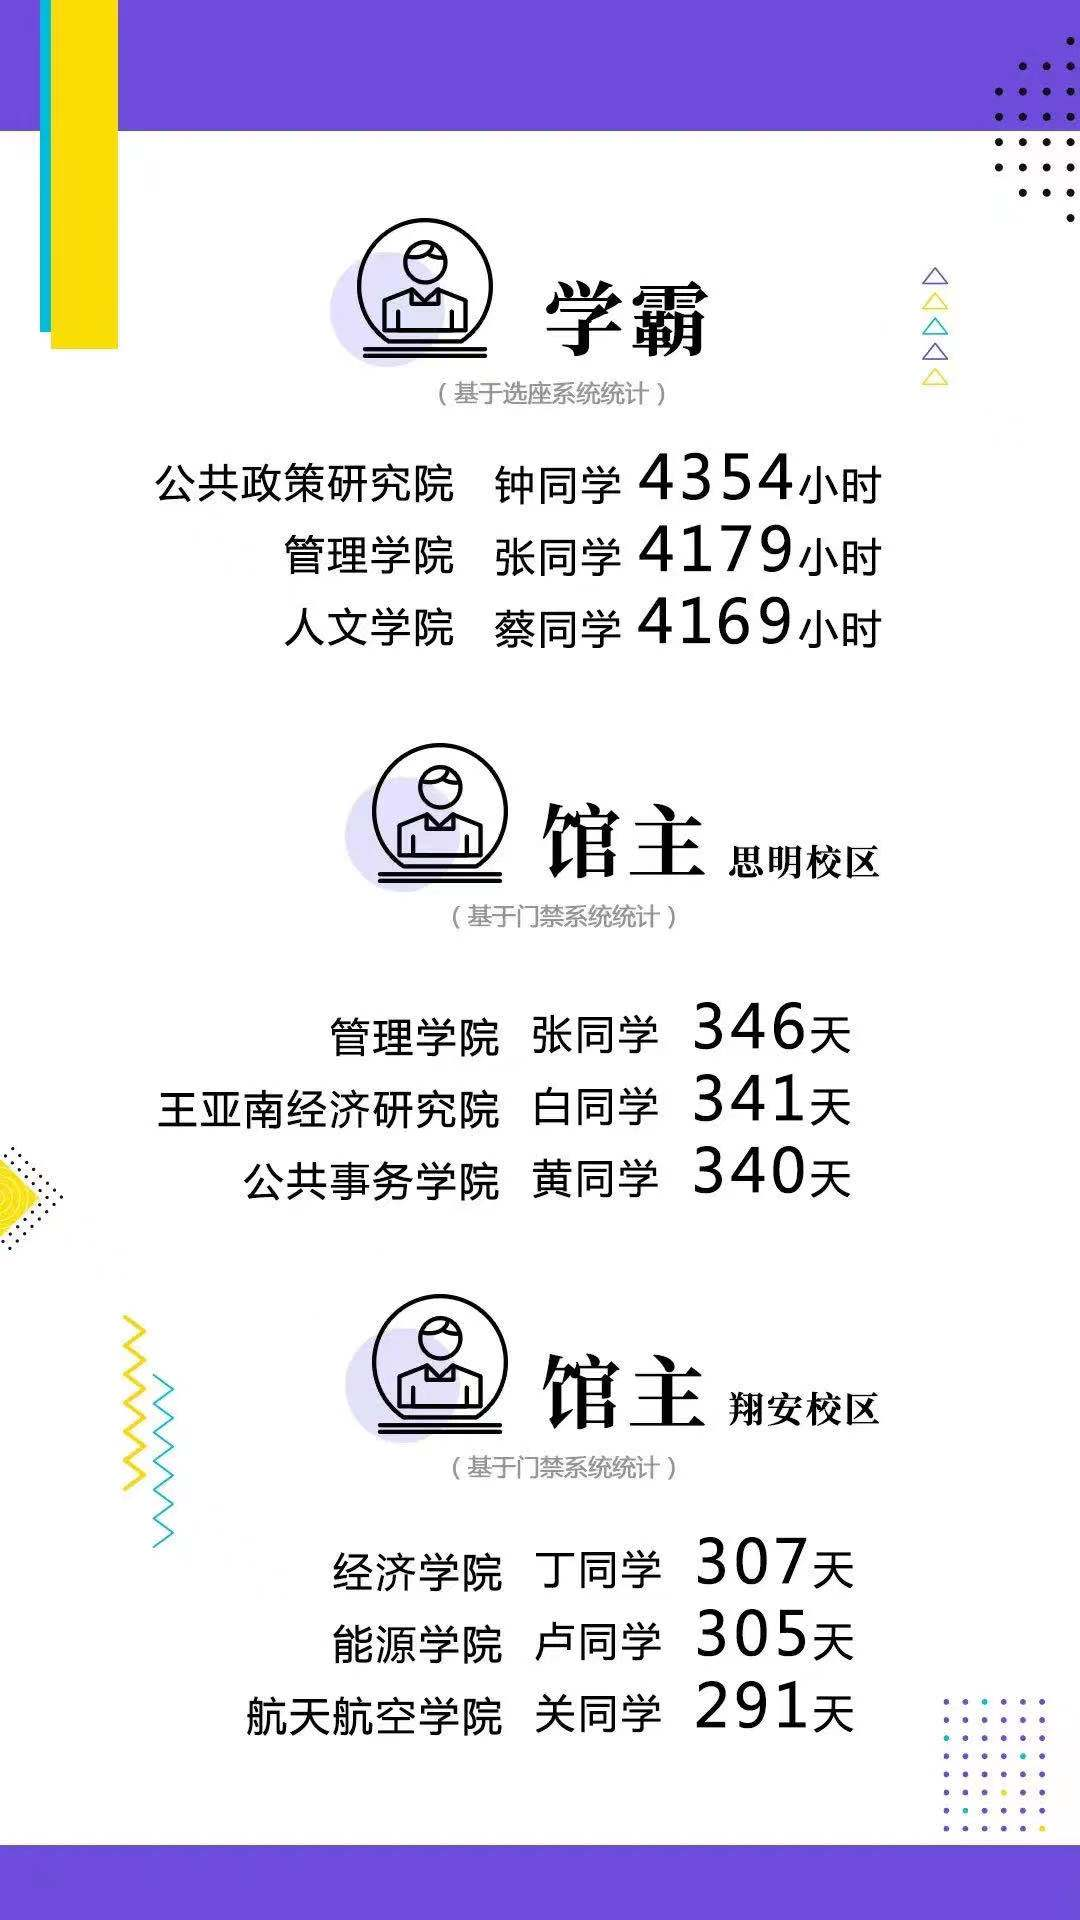
\includegraphics[width=.75\linewidth]{liblord.jpg}
% 	\caption{我是馆主}
% 	\label{fig:liblord}
% \end{wrapfigure}	

与此同时,我还要感谢厦门大学以及厦门大学图书馆。
% 厦门大学在我硕士求学期间免去了我所有的学费,因此为我提供了一个非常舒适的生活条件,对此我表示衷心的感谢。此外,厦门大学图书馆给予了我一个安静的研究环境,让我可以静心的想问题和看书。这种感激之情难以言表。

% 我想,\reffig{fig:liblord}足以反应我将对厦门大学图书馆有多大的感激。

此外,我还想感谢我妈家对我各方面的帮助。

最后,我还想感谢我爸。我爸为我付出了很多。我爸也一直支持我继续学习,对此我表示感谢。

本人实在不善言辞。我只能用我接下来的努力,在某种意义下来继续感谢各位。
\newline
\newline

\hfill {\fontsize{55}{60}\selectfont\bfseries\kaishu 关劼文}

\hfill{\today 于厦大图书馆}

\end{ack}
